\documentclass[12pt,twoside]{book} 
\usepackage[toc,page]{appendix}
%\usepackage[left=2.5cm,top=3cm,right=2.5cm,bottom=3cm, bindingoffset=0.5cm]{geometry}

\usepackage[paperheight=9in,paperwidth=7.5in,top=1in,bottom=1in,right=1in,left=1in,heightrounded,showframe, bindingoffset=0.5cm]{geometry}
\usepackage[font={small}, labelfont=bf]{caption}
\usepackage{subcaption}
\usepackage[utf8]{inputenc}
\usepackage{setspace}
\doublespacing
\usepackage[dvipsnames]{xcolor}
%Font
\usepackage[T1]{fontenc}
\usepackage{booktabs}
\usepackage{fouriernc}
\usepackage{quotchap}
\usepackage{cancel}
\usepackage{titling}
\usepackage{gensymb}
\usepackage{imakeidx}
%\usepackage[english]{babel}
\usepackage{fancyhdr}
\pagestyle{fancy}
\fancyhf{}
\fancyhead[LE,RO]{\leftmark}  %headers
\fancyhead[RE,LO]{A Numbers Game}
\fancyfoot[CE,CO]{\thepage}
\usepackage{graphicx}
\usepackage{amsmath,commath,amssymb,amsthm,blkarray}
\newtheorem{theorem}{Theorem}[chapter]
\newtheorem*{claim}{Claim}
\usepackage{mathtools}
\usepackage{titling}
%\setlength{\columnsep}{1 cm}
\usepackage{esvect}  %to make vectors in another way
\usepackage{siunitx}
%\usepackage[section]{placeins}
%\numberwithin{equation}{chapter}  %ch.eq#
%\numberwithin{figure}{chapter}
\newcommand{\imp}[1]{\textbf{#1}}
\renewcommand{\vv}[1]{\mathbf{#1}}
\usepackage{mathrsfs}
\usepackage{physics}
\usepackage[tikz]{bclogo}
\makeindex[columns=2, title=Alphabetical Index]

\begin{document}

		\begin{bclogo}[couleur=MidnightBlue!2!white, arrondi=.645, logo=\bcvaletcoeur , ombre=true,epOmbre=.28,couleurOmbre=MidnightBlue!29, barre=none, nobreak=true ]{} \vspace{-2ex}	\centering\Huge The Art of the Prediction:\vspace{.5cm}  How to (Probably) Predict the Future\\[\baselineskip]	{\Large{DataTeam6}}\\ % Author name
		{\large{ December 4th, 2018}}
	\end{bclogo}
%	\pretitle{%
%		\begin{center}
%			\LARGE
%			%\includegraphics[width=10cm,height=10.7cm]{subtitle}\\[\bigskipamount]
%		}
%		\posttitle{\end{center}}
%	\title{It's All in the Numbers: How to (Probably) Predict the Future}
%	\author{Data Team Six\\
%}
%	\date{}
	%\titlehead{\centering\includegraphics[width=6cm]{figure}}
%	\maketitle
		\vspace*{3in}
		%\begin{center}
		%	\includegraphics[width=\textwidth]{subtitle}
		%\end{center}
	\tableofcontents
		\begin{savequote}[45mm]
			Insert dramatic quote here.
			\qauthor{Person}
		\end{savequote}
	\chapter{Introduction}
	The second law of thermodynamics states ...  This is often regarded as the pillar of modern physics, the one rule our universe must obey.  A natural, and valid, interpretation of this law is that we live in a chaotic, random world.  And our daily experiences reflect that.  There are billions of people, thousands of languages, hundreds of variations of cola. Adding in mother nature and her tendency to throw all kinds of curveballs leads to tremendous amounts of disorder, it is difficult to imagine how we are able to live in such a complicated world.  
	
	Yet, for all the randomness and complications, we have become remarkably adept at muddling through the chaos, at predicting what comes next.  Even without a gift of premonition, I can largely tell how my day will go, what I will eat, when I'll finish work. I can tell what adding just the right amount of olive oil will do to my dish, without any exact measurements. With the assistance of my peers, my predictions can delve even deeper. I can predict what route to take based on the traffic, what to wear based on my weather man, which game to watch based on sports analysts, and so on.  So how have we become so good at prediction?  How can we predict finer details, such as traffic patterns, market fluctuations, or health scenarios?  Well, the answer (often) lies in the numbers.
 
 Before we begin, I just want to mention that we will mainly be looking at numerical prediction techniques.  There are certainly limitations to this approach, as we all know.  Regardless of how tried and true  any recipe may be, my grandmother made a better spanokopita with her ``just right'' approach.  And she was remarkably consistent in her results.  Gut reactions still dominate our world, especially as the stakes get higher.  Statistics may tell you that it is unlikely that you will be attacked by a shark, but I'm still wary (I'd like to think understandably) on most beaches.  
 
 The value of human instinct and intuition is incredibly valuable and that will not be disputed. And at times in the book, we will see where statistical thinking came up short.   However, we want to explore areas where humans turn to their pens and computers to aid their prediction abilities, and areas where even with the aid of high powered computing, we still are blissfully unaware of what comes next.

	\begin{itemize}
		\item Anecdote about cooking, recipes, etc.
		\item Companies use analytics when they decide what movies to air, ie \emph{The Iron Giant} or \emph{Steve Jobs}
		\item The history of quantitative predictions, from the Greeks earliest attempts to today's world of big data.
		\item Emphasize where human intuition is still valuable, business, sports, weather, etc. 
		\item The main theme of the book is how we use tools to predict what is going to happen next, ranging from quantitative tools, which are the most prevalent, but not forgetting human intuition, which is most prevalent in the Drake equation, stock markets, sports, and gambling markets. Hopefully sprinkle in anecdotes to make the more technical aspects more approachable, perhaps include some code.
		\item German tank (super cool)
	\end{itemize}
	\chapter{Differential Privacy}
		\begin{savequote}[45mm]
		Vincent, you can hop in here.
		\qauthor{Person}
	\end{savequote}
	\chapter[The Drake Equation]{Are We Alone?}
	For as long as humans have been around we have looked up and wondered whether we are alone. 
	And, to date, we do not know the answer to this question.  Granted, there are many, many stories of alien encounters, tales that have become increasingly far fetched over the years, but no proof of extraterrestial life has ever been found. So, despite what many believe, we have no way of knowing for sure whether or not we really are alone in our universe.  Hell, we don't even know if our universe is the only universe\footnote{Many physicists believe in a ``multiverse'' theory, which proposes for all intents and purposes an infinite number of universes, and ours is simply one of the many}. So, can we predict when we will meet our terrestial neighbors, if they do indeed exist?  Not really.  But we can predict if there \emph{is} life out there.  Well, kind of.  
	
	How do we go about predicting the existence of extra-terrestial life?  Insert the \imp{Drake Equation}. We'll begin our story in 1961 at the Green Bank observatory\footnote{ Frank Drake hosted a conference in 1961 on the search for extra-terrestial life.  Green Bank was an ideal gathering for different astronomers.}, a radio telescope located, rather unsurprisingly, in Green Bank, West Virginia.\cite{GreenBank} Green Bank is a town that seems out of place in 2017. For one, the town has a population of 143, and perhaps even more shockingly, the town prohibits the use of cellular devices.  Yes, you read that right.  
	
	The Green Bank observatory was where Frank Drake\index{Frank Drake} presented his now famous Drake equation\index{Drake equation}.  The equation was presented at a conference and intended to answer the ``are we alone'' question from a probabilistic standpoint, providing a range of the number of intelligent alien species in our galaxy, which can more or less be extended to our universe by multiplying by the number of galaxies in the universe\cite{numgalax}\footnote{Estimates put this number in the trillions} Furthermore, the question tried to answer not only if there is \emph{life}, but if there is \emph{intelligent} life.  While this sounds impossible to do with a series of fractions multiplied together, the equation does indeed shed some quantitative light on the question.
	
	In all it's glory, we have reproduced the Drake equation below:
	\begin{equation}
	\boxed{\boxed{N=R\vdot f_p\vdot n_e\vdot f_\ell\vdot f_i\vdot f_c\vdot L}}
	\end{equation}
	What do all these variables mean? 
	\begin{itemize}
		\item 	$N$ is the number of civilizations in our galaxy that are within our ``light cone''\index{light cone}.  That is, the number of civilizations that we would be able to detect if they do exist.  This is an important distinction, as there could very well be civilizations that exist, but if we cannot detect them, we are no closer to our answer than when we started. 
		\item $R$ is the rate of formation of stars, or how long it takes the average star to form in our galaxy.  This is important because it typically takes stars billions of years to have the capability of supporting life, and given that the universe is estimated to be around 14 billion years old\cite{universeage}\footnote{13.8 billion years to be exact}, this limits the possibilities of life formation dramatically.
	\cite{space.com}  
	\item $f_p$ is the fraction of those stars that develop planetary systems, which is an obvious pre-requisite for life (as far we know). Now it is starting to become clearer how the equation works, as we will keep multiplying fractions together to get a final probability, or better a range of probabilities (more on that later).
	\item $n_e$ is the number of planets in a solar system with an environment suitable for life.  In our solar system, there is one obvious answer, Earth, but there are speculations that both Mars and one of Saturns's moons, Enceladus\cite{lifenasa}.  Now, if we have life on moons, we have to include this, as nomenclature ultimately does not affect life.
	\item $f_\ell$ is the fraction of suitable planets that life actually appears.  In our solar system, out of the potentially habitable planets, only Earth is known to have life (otherwise this whole endeavor would be a waste of time).  
	\item $f_i$ is the fraction of life bearing planets on which intelligent life emerges.  There's always one wise guy who'll say zero, but this question is actually quite difficult to answer. Given that there is intelligent life on Earth, our default answer would be 100\%, but since only one or few species out of the billions developed intelligence, that this percentage is extremely low, and in fact close to zero.  We, as humans, tend to fancy ourselves as the only intelligent beings on Earth, and there is a valid argument to be made for that, but many will argue that other animals, such as dolphins and whales\footnote{In case you do not believe this, on the Internet there are videos of whales hunting seals that will probably change your mind}  exhibit signs of intelligence\cite{dolphinssmart}   This will change the probability of intelligent life existing dramatically.
	\item $f_c$ is the fraction of civilizations that develop their technology to a point that they can communicate, or at least convey their existence into the galaxy, and thus make themselves detectable.  Again, there could very well be life, but if we cannot see it, it is no good to us.  Perhaps there are alien creatures in our galaxy asking the same questions, unaware of our existence.
	\item Finally, $L$ is the length of time that civilizations last, or, more accurately, the length of time they transmit messages into space.  As humans, we have been transmitting our electromagnetic waves\cite{eandm} waves into space since the late 1800's with the invention of the radio.  Now, that means we have been roughly transmitting our existence for about 100 years, give or take.  Therefore, the $L$ for Earth would be about $100$. How long will our civilization last?  Hopefully a while, we can all probably agree on that. Realistically, however, there is a pretty wide range on how long people think we will last, ranging from the very cynical (less than a hundred years) to the very ideal (millions of years). This range again makes the range on the number of civilizations that could exist in our galaxy fairly dramatic, as we shall shortly see.	
	\end{itemize} 
	
	Now, comes the tricky (and fun) part; crunching the numbers.  Be warned, the final result will not be a definitive answer as to how many alien civilizations are out there, it will not tell us if they benevolent, nice, maybe even funny good hearted creatures, or cold, malicious monsters hell bent on our destruction.  For that, it is probably best to delve into your science fiction collection and decide for yourself.  Rather, the Drake equation will yield a wide range of possibilities for the number of civilizations.  To do this, we bring in doctor Jeremy Carlo, professor of physics at Villanova, and an amateur astronomer, who has presented on the Drake equation numerous times. With Dr. Carlo, we will go through an example of the Drake equation, and find that, based on different people's beliefs, that it will indeed yield a tremendous range of possibilities concerning the existence of intelligent alien lifeforms in our galaxy.
	
	What the Drake equation essentially tells us then, is that we either are alone in our galaxy, or we are one of countless number of civilizations, with every possibility in between.  So, while it is a fun exercise, the Drake equation is not necessarily telling us anything we did not already know.
	\chapter[Quantum Mechanics]{Dead and Alive? An Introduction to Quantum Mechanics}
	\begin{itemize}
		\item Transition to another science related topic
		\item Talk about probabilistic nature of nature.  We can never really predict \emph{exactly} what is going to happen next, so our best bet is to \emph{guess}, using probabilistic methods.  
		\item Fenyman diagrams, quantum tunneling, probability amplitudes, real world applications such as \imp{quantum computing}, perhaps its own section.  Schr{\"o}dinger's cat, Heisenberg's uncertainty principle, the two slit experiment.  Introduction to multi-verse theory, etc.
		\item Generalize quantum mechanics to a more macroscopic scale, how the models built in quantum mechanics have worked very well in their macroscopic predictions.  Perhaps a section on \imp{modelling} in general, and how mathematical models are used to explain what we do not know, to predict what is to come, but are not necessarily the end all be all.  
	\end{itemize}
	\chapter{Statistics and Probability}
	\begin{itemize}
		\item Talk in this section about probability, and how modern computing is in many ways indebted to probability, see Alan Turing and Enigma code breaking.  
		\item Introduce classical, frequentist statistical thought, and Baye's rule, and how they affect our way of thinking about future events
	\end{itemize}
	Anybody who wants to delve into the art of prediction would be wise to acquaint themselves with statistics.  This probably is not anything that most have not heard before, and is certainly much easier said than done.  
	
	While Bayesian and frequentist thought are often at odds to say, it is often pivotal for models to consider both fields when making their predictions.
	\chapter[Rise of the Bots]{Artificial Intelligence: What We can Learn from Tay Bot}
	\begin{itemize}
		\item In this chapter, we discuss how artificial intelligence is built off one thing: \emph{Data}, and lots of it.
		\item Talk about how machine learning using artificial networks is really a means of predicting how humans act, and if this can be emulated by computers, essentially simulating intelligence
	\end{itemize}
	Artificial intelligence.  The singularity.  Keanu Reeves.  Where to start?  What is artificial intelligence?  Are we doomed?  Aren't computers already smart?  Can we live forever?  When is this going to happen? These are questions that are commonly associated with artificial intelligence, and while we will certainly answer them as well as we can without diving too deep into philosophical waters, we would also like to explain some of the underlying theory behind machine learning, and ultimately how it connects to predictive analytics\footnote{In a nutshell, artificial intelligence is predictive analytics}.  
	
	Whenever artificial intelligence is mentioned, a sense of fear tends to take hold of people.  Perhaps influenced by popular movies such as the Terminator, or the Matrix, where our former friendly computers realize humans make better batteries than conversation, there is a legitimate fear in many about a one-day \imp{singularity}\index{singularity}. What is the singularity?  Broadly speaking, it is when computers will become sentient.  By this interpretation\footnote{By no means the only, or even the correct interpretation}  a computer will be cognizant of its existence.  Why does this matter?  Well, computers, with their incredible speed, processing power, and memory dwarf humans in computational ability.  But, until recently, they could not think for themselves.  They could not create.  Computers were programmable, and thus only as smart as their creators made them.  Recently, however, computers have been able to ``learn'' from their mistakes, and exhibit signs of intelligence. Or so we have been told.  
	
	The argument is that, eventually, these computers will think like humans, that is humans with nearly infinite knowledge and processing speed that not even transcendental geniuses the likes of Isaac Newton could not even fathom\footnote{My apologies to Gauss, Euler, etc.}. And, eventually, the computers will move beyond their programming, or so it is theorized. In theory, computers will be able to accelerate their learning at incomprehensible speeds, due to the processing power and memory capabilities they are endowed, and technology will increase so rapidly, that the human mind cannot imagine where it will lead.  This belief is more technically what is meant by \emph{the singularity}, and it is this definition that is often accompanied by fear and bewilderment among people\footnote{Well known scientists have expressed their reservations, to put it mildly, about artificial intelligence, such as acclaimed theoretical physicist Stephen Hawking\index{Stephen Hawking}}, thanks at least in part to doomsday predictions in movies, books, television and so on. But is their fear justified?  Will we meet our fiery doom at the hands of our metallic counterparts.  Well, in accordance with the central theme of this book, \emph{probably} not.  
	
	Artificial intelligence, (like machine learning) is in many ways just a buzz-word.  Later we will go into more detail into the algorithms behind ``machines learning'' but for now it suffices to say that computers aren't really smart.  Just ask Alexa or your google assistant any (insert specific question that actually stumps google).  What computers are doing is \emph{recognizing}. The crux behind ``deep learning'' is that computer programs are fed in lots and lots of data and eventually recognize patterns, an imitation of true learning.  Imagine a child (cousin) seeing their first hawk.  His mind classified all birds as hawks (the way we classify a hawk as a bird)  All birds are now hawks until his brains begin to process higher. This is why image recognition, for example has evolved significantly in the late 0's and 10's (really would have thought we could have come up with a name for these decades by now.  Worry not, the twenties are soon upon us.)  
	
	While this sort of computer recognition software, given enough data, can lead to what may resemble human intelligence, it really isn't.  While it is a step-up from the if-else programming that has dominated programming for the vast majority of its history, it is still not intelligence.  However, it does have some scary problems.  Recognition learning often does not rely on parameters (more on this in the chapter on self-driving cars), ie the models do not necessarily ``mean'' anything.  Traditionally, for prediction problems, statisticians, psychologists, baseball teams, and many more fit a straight line to a graph between their desired outcome (y-axis) and what they believe is a variable that should be related to it (x-axis).  A simple example is expressed in figure \ref{figurebaseball}.
	\begin{figure}[h]
		\centering
		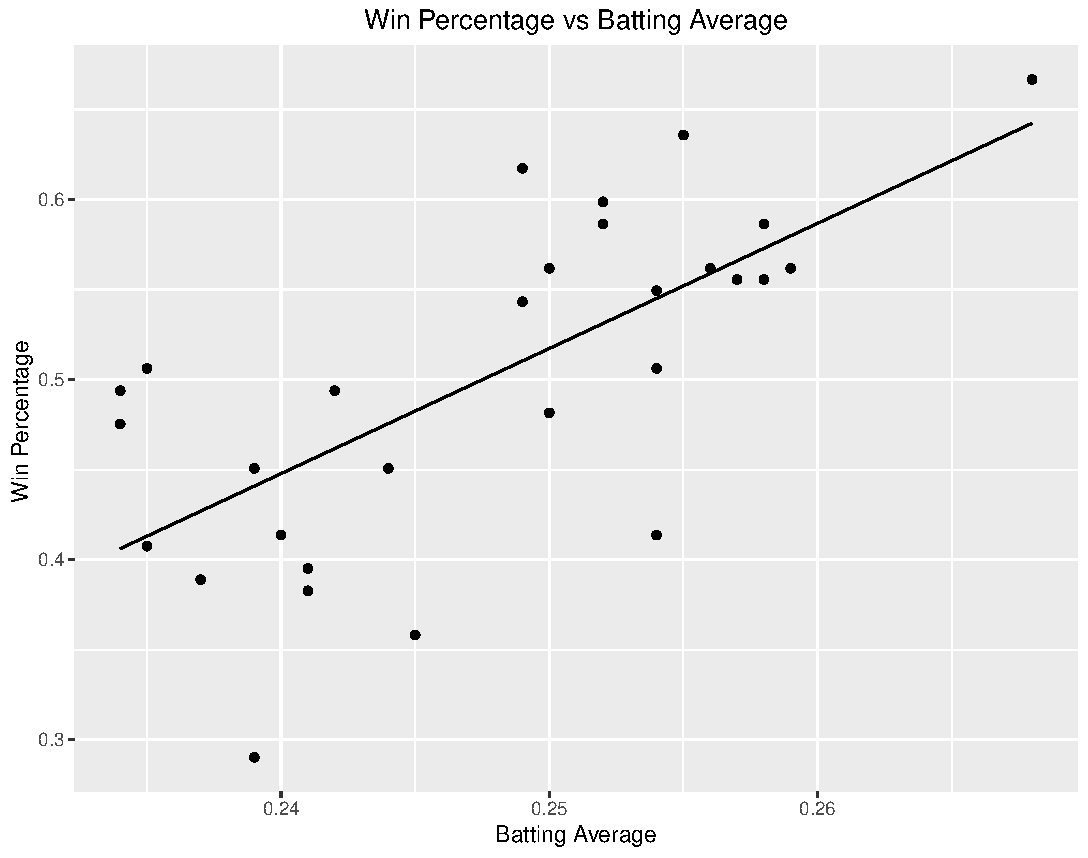
\includegraphics[scale=0.5]{baseballpic}
		\caption{Team wins vs batting average, MLB 2018}
		\label{figurebaseball}
	\end{figure}



	\noindent\rule{3cm}{0.6pt}
\\

\vspace{-1.25cm}
\noindent\rule{3cm}{0.6pt}  \textbf{Technical Sidebar}


**Include some details from regression 530 notes, OLS, matrix form, and confidence bands**


\setlength\parindent{9cm}\rule{3cm}{0.6pt}
\\

\vspace{-1.25cm}
\setlength\parindent{9cm}\rule{3cm}{0.6pt}

\setlength\parindent{.75cm}
	
	We interpret our regression result as a 10 point increase in team batting average (.300 to .310) increases a teams win total by 6.95\%.  Since there are 162 games in a season, 11.26 wins better.  Obviously, from the graph, this regression is rather meaningless, and we have several metrics and methods to back this up.  ($R^2=0.45$, histogram, assumptions etc.)  If we extrapolate this to the point where a team has a batting average of 0, then we predict a team would win -2 games, which obviously makes no sense.  Therefore, it would not necessarily be our best predictor.  Of course, we can include more variables and do a multiple linear regression, which could improve our model, and while the interpretation is not quite as cut and dry, especially since we may need to scale some variables.  We can't just plot the regression as easy anymore, as we have multiple x-variables (although we can still compare our output to our a teams winning percentage, the ``y'' variable).  
	
	This regression still does have real, physical parameters that can be explained if we are careful and think it through.  In fact, linear regression is an old and well researched and developed tool, with established methods to verify the validity of results and optimize results (ie which variables are most effective to best predictions, or fitting confidence intervals around our line of best fit, prediction bands etc).  
	
	An ``artificial intelligence'' method, such as a regression tree or a neural network, on the other hand, would likely yield better prediction on a teams final win total.  Given enough data on past winning teams, we can train these models and then use the trained version of the model (with all the trained weights in the case of the neural nets) to predict the current year (2018) and compare it to actual results.  
	
	Likely, this will yield better accuracy by different statistical metrics (MSE, etc.), which is useful.  However, it may not \emph{mean} anything.  And therein lies the problem with these new computer ``learning'' methods.  The neural network, for example, may weigh certain variables of interest heavier or lighter based on how they have predicted in the past, in a way linear regression is unable to.  How often are things linearly related, or even related by some obvious function?  Probably not very.  But, the machine learning methods do not tell us why variables are important, or how they specifically lead to our desired result.  And just relying on that answer could be dangerous if we do not know why it works.  A baseball team may use the output, despite its lack of clear reasoning, because of its predictive power, but then regret the decision when a drastic change in the game renders the results from the neural net/decision tree regression useless.  
	
	For example, in 2016-2017, players (from the advice of sabermetrics) decided strike outs were okay, and decided to live by the ``elevate-celebrate'' motto.  Home runs were at a record high[cite].  This paradigm shift in the game would not have been present in the past data, so the non-parametric predictions now lose some of their shine.
	
	\chapter{Financial Markets}
	
	\chapter{Amazon's Crystal Ball}
	\begin{itemize}
		\item Talk about how different companies, like Amazon, use data to give you the best possible buy.  They predict what you want next, and lure you to buy more.
		\item Talk about the selling of data by companies like Google to outside advertisement agencies, and how effective these advertisement ventures are.
	\end{itemize}
	\chapter{Yup More Amazon.  This time its logistics.}
\begin{itemize}
	\item After finishing my freshmen year of college, and again at various points throughout the next three years, I worked at a Coca Cola distribution plant.  My job was to help deliver soda to small market stores in Southeast New Hampshire, in an area that covered roughly 300-400 thousand people (think the Manchester metro, if that helps.  It probably doesn't.)  Despite not servicing a huge market, mainly delivering to gas stations and restaurants, and basically any store that ordered coca cola products but wasn't a supermarket or fast food chain, it still was an enormous undertaking.  
	
	We had approximately fifteen trucks going out daily, each making 15-20 stops with 300-500 cases.  Most cases carried between 8-24 bottles, so on average each truck had roughly 6000 bottles or cans on board a day.  The distribution plant, located in Londonderry NH was enormous, and that was not including the production center attached.  Trucks would drive in all day and night long, some coca cola trucks, others from other companies.  The sheer size of the operation was astonishing.  And it ran (contrary to what we'd say on the truck or in the warehouse) relatively smoothly?  How could this be?
	
	Logistics.  Our world is very inter connected, with the global trade market bigger than ever before.  In order to keep everything running smoothly, a complicated and thorough logistics system is required.  Starting at the smallest levels, these logistical situations can be solved by man power.  But moving up levels in the distribution size increases the nightmare.  Distributing a lot (but not all) of the soda and water to small stores in southeastern New Hampshire requires a well orchestrated effort that is inevitably heavily tied to computing solutions.  
	
	Orders are placed by sales representatives, who (assuming customers do not place their own orders) visit stores and make an educated guess as to how much to order.  At the sales representatives disposal is a wealth of data on that specific accounts past orders, giving the sales rep more insight into what order to place.  However, things get complicated after here.  Sales reps will place about 20 orders a day, so the combination of all the sales representatives makes for hundreds of orders to be put together.  Already, the complications are adding up.
	
	The orders are sent through a computer system, which tells which orders to get.  The product is made continuously as various products are put together on palettes, for efficiency.  Picked by workers, then palettes built.  Trucks set up based on computer, safety, height, when customers want order, algorithms, but manager ultimately decides with aid of interactive software. 
	
	This is an increasingly automated field, but one that is do-able with human interaction. Sales can be made without immediately available data (albeit data is probably in the back of a sales reps head).  Managers and drivers have discretion over when to do stops and such.  But these routes are usually the same week to week.  There is a familiarity between driver and account.  The product, despite having many different flavors and variations (there are more than 12 ways of selling classic coca cola), still belongs to one family of product.  While computers aid, the logistics at the company I worked at were somewhat solvable without the aid of too much algorithmic thinking or the aid of computing solutions.  
	
	Ramp up operations to another level, however, and the logistical challenges grow even greater.  Imagine a company offering to send you virtually any item imaginable within 2 days with the click of a button.  Yeah, our old friend Amazon gets two chapters.  We recently talked about the software side of Amazon, and how their algorithms and data analytic techniques allow them to buy more and more.  But how exactly do they get their orders so fast?  No, not drones.  Not yet at least.  
\end{itemize}
	\chapter{Trying to beat Vegas?  Don't Bet on it}
	\begin{itemize}
		\item How the odds work, your bet changes the odds, because so many knowledgeable people gamble, like the stock market, the Vegas lines tend to be pretty accurate
		\item Your options?  Be better than the market, or you could find a loophole
		\item Talk about Leicester City, the soccer team with 5000-1 odds to win their division$\ldots$ that won their division.
	\end{itemize}
	\section{The Math Behind Gambling}
	Buchanan stuff
	\section{Even Bookmakers make Mistakes}
Prior to the 2016 Premier League season, Leicester City was given 5000-1 odds to end the season with the best record by English bookmakers William Hill and Ladbrokes\footnote{Technically not Vegas, but still a gambling bookmaker}. That means a bet of 10 dollars on Leicester, perhaps a tradition you have followed your whole life, would net you 50,000 dollars.  The reward alone makes the 5000-1 odds even harder to believe.  Unless you believed Leicester City had absolutely no hope of winning the league \footnote{Elvis Presley being found alive had the same odds as Leicester City winning the Premier League in 2016.},\cite{leicester} a 5000-1 odd would make sense to bet on, as even a very small bet (read: low risk) could reel in a substantial reward.  So, the question is, why was Leicester rated so low?

Leicester City Football Club, otherwise known as the Foxes, is a British football roster that, until recently, was a franchise rife with disarray, disappoint, and, at best, mediocrity.  In its 133 year history, Leicester had never won the Premier league, or its predecessor Division One.  Not once.  Even the Cubs, the lowly Chicago Cubs only took 108 years between their championships.  Worse yet, Leicester only finished \emph{second} once, and that was during the 1928-1929 season.\cite{Leicester2}  And, to make matters worse, the Premier League, like many other high level soccer leagues, has been lacking in parity amongst its teams for years on end.  Manchester United, Manchester City, Arsenal, and Chelsea year after year attract top players, and almost always seem to come on top. And finally, to compound the issue, Leicester City came off a miserable 2014-2015 campaign, finishing fourteenth out of twenty teams, only escaping relegation\footnote{Relegation is when teams that finish at the bottom of the Premier league are ``relegated'' to a lower league the next season} with seven wins in their final nine games.\cite{Leicester3}  
The hot finish, however, did not translate to optimism in bookmaker's minds, in part due to skepticism of the talent on the roster and the sacking of manager Nigel Pearson.

Astonishingly, however, Leicester City got off to a hot start in the 2015-2016 season. Striker Jamie Vardy\index{Jamie Vardy}  led his team's tremendous effort in the early season, and Leicester City jumped to the top of the Premier League by Christmas day of 2015\index{leicester5}
.  While many were skeptical at first of the squad's hopes, the team became an international sensation as more and more people became aware of what was going on.  The team with 5000-1 odds was looking more and more likely to win it all.  Instead of tailing off, Leicester maintained their grip on first place.  On May 2, 2016, Leicester City secured the Premier League championship, in the process making some lifelong fans a lot of money, and destroying conventional wisdom in betting. \index{Leicester4}

Unfortunately, lightning did not strike twice, as the club's success was short lived, with the 2016-2017 season falling in line with what was expected of the surprising 2015-2016 campaign. The season ultimately saw the removal of Claudio Ranieri, the (at one point very popular) manager that brought Leicester the title the season before, on February 23, 2017.\index{leicester6}
\begin{table}[t!]
	\centering
	\begin{tabular}{ll}
		\toprule
		Event                                     & Odds    \\ \midrule
		Leicester winning  Premier  & 5000-1  \\ 
		Hitting a Hole in One                     & 3632-1  \\ 
		Fatally Slipping in Shower                & 2232-1  \\ 
		Dying as a Pedestrian                     & 672-1   \\ 
		Catching Ball at MLB game                 & 570-1   \\ 
		Having a Child Genius &261-1 \\ 
		Getting on Plane with Drunken Pilot       & 117-1 \\ \bottomrule
	\end{tabular}
	\caption{These are things more likely, statistically to occur, then the odds bookmakers gave Leicester City to win the Premier League title in 2016\cite{leicester7}}
	\label{tab:leic}
\end{table}
\section{On the Average, You'll Lose}

Ostensibly, the conclusion from Leicester City is to bet on the underdog.  Well, not really.  If there is data suggesting that Leicester city was greater than a 5000-1 odd, which they obviously were, then the bet makes a lot of sense.  If your individual odds are different from the bookmakers significantly, it is best to jump in\footnote{Not advocating for gambling, just speaking from a mathematical sense}.  However, people tend to know less than Vegas bookmakers.  While Leicester City is a tremendous story, one that will undoubtedly be told for a while, glorified in the movies, it is an exception.  For example, even the lowly Cleveland Browns, the franchise that's toiled in obscurity for decades, and who had only 3 wins in the previous 2015 NFL season, started the season with 150-1 odds, a number not nearly as drastic as Leicester\cite{leicester}.  


 As evidenced by the data, the best advice, no matter how hot you are, no matter what dream you had, no matter what socks you're wearing, is to quit when ahead.  Many have learned the hard Vegas welcomes avarice as an old friend. The chances of beating the market consistent are slim, and attempting to do so can have catastrophic consequences. 
	\chapter{Predictive Analytics in Sports}
	\begin{itemize}
		\item Begin with baseball, then basketball.  Talk about the players that care, that ones that don't, front offices, and coaches takes on statistics and quantitative predictions in major sports.
	\end{itemize}
	It is 
		\chapter[``Machine Learning'']{Self Driving Cars:  How the Chain Rule will Rule our Roads}
		
		Admittedly, this is a misleading title.  Self driving cars are not solely reliant on the chain rule from calculus.  But is a fundamental aspect of neural networks, the basis for self driving cars and many recognition problems.  
		
		
		When you hear machine learning in the news, it is important to note that the machines are not really ``learning'', at least in the sense you are probably thinking.  Rather, what computers are essentially doing is recognizing a pattern and acting on it.  
		
		Now, we are going to go through an example with python and R.  Using neural networks, we will ``teach'' our computer how to correctly identify the handwriting of various people.  In essence, the secret to our success will rely on how much data we have; neural networks rely and thrive on data  (this is why google dominates so many machine learning competitions).  We will also do this project in R using random forest (Vince has part 1 I have part 2)
		
		In addition to neural networks, there are other methods (probably a little more intuitive) that are more robust in certain situations.  I mainly am referring to tree based regression methods.  Insert diagram/explanation of boosting.  Also mention BART and random forest.  
		
		Tree based methods tend to be better with noisier, but ``simpler functions''.  For example, random forest classification will not perform as well in handwriting recognition (as we saw), but it would likely do better in predicting stock market futures [cite].  Neural nets, with sufficient data, do well with complicated, low noise functions, hence their dominance in recognition problem (ie spotting a cat in grass).  
	\chapter[When the Numbers Lie]{Where Math Doesn't Tell the Whole Story}
	\begin{itemize}
		\item Can essentially go through every previous topic and show examples of data analysis ``making mistakes''.
		\item Advocate for predictive analysis to still need human intuition, not just mathematics.  This is something that is easy to explain with financial markets and baseball, but is clearly more difficult to do with the sciences, such as physics or chemistry.
		\item Talk about the limits of mathematical models, how they are not impervious to initial conditions, especially those subject to mathematically chaotic behavior, reference figure \ref{fig:chaos1}. The Python code to create these graphs is included in the appendices.
		\item The most common example is the ``butterfly effect'', often used to help explain why the meteorologists do not always get it right, and how astonishing it is that they can even tell us anything, let alone often give accurate predictions.
	\end{itemize}

\begin{figure}[ht]
	\centering
	\begin{subfigure}{.5\textwidth}
		\centering
		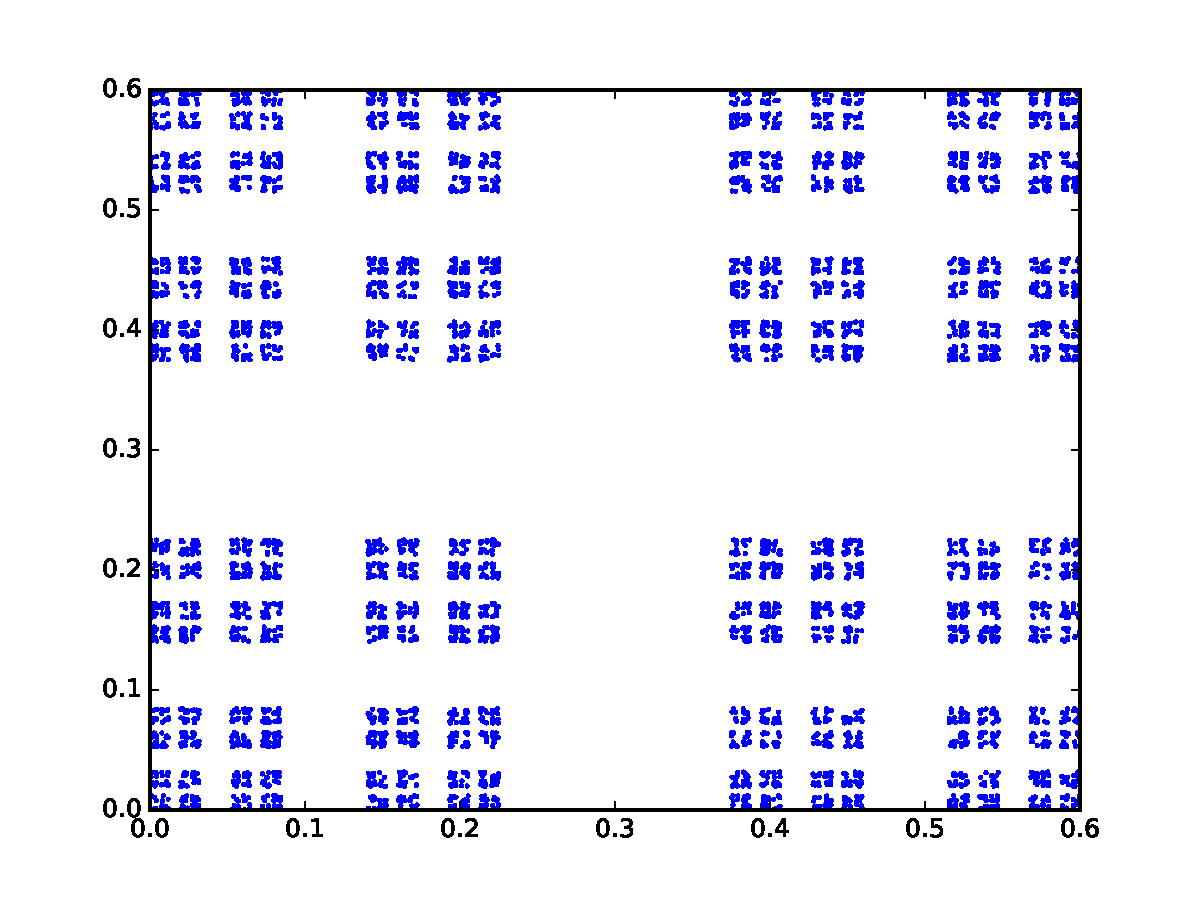
\includegraphics[scale=.35]{chaos2}
		\label{fig:chaos2}
	\end{subfigure}%
	\begin{subfigure}{.5\textwidth}
		\centering
		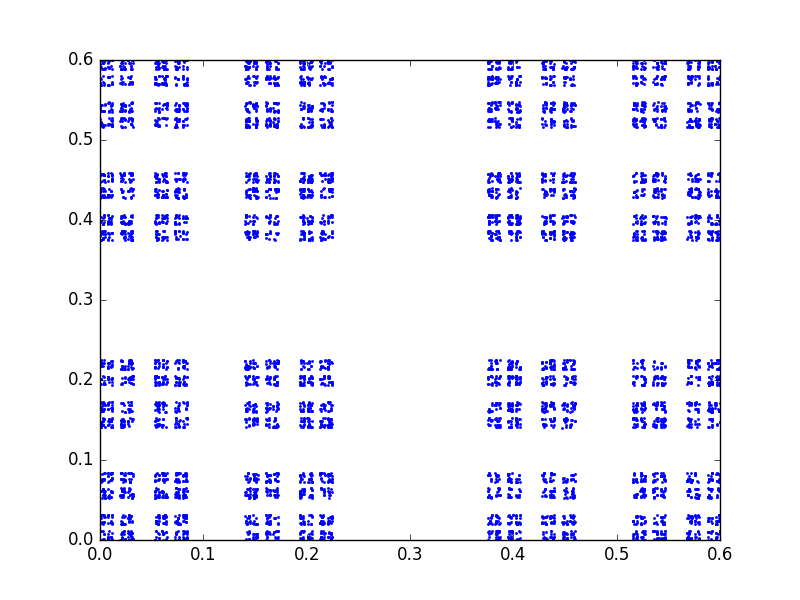
\includegraphics[scale=0.35]{chaos1}
		
	\end{subfigure}
	\caption{Left:Notice this is chaotic and seemingly random.  If we start with a square and a point somewhere in the square, and randomly go one half of the distance between a current point and one of the four quarters (randomly chosen, we could use a dice and only consider the numbers 1 to 4 for example, with each number corresponding to a specific corner of the square), and do this thousands of times, we get this graph.  Now, if instead of traveling halfway to the corner rolled, we travel 3/8 of the way, this nice picture appears, seemingly unrelated to the figure on the left}

	\label{fig:chaos1}
\end{figure}
	\begin{appendices}
		Python codes, technical explanations behind the quantum mechanics section, etc.
	\end{appendices}
	\clearpage
	\begin{thebibliography}{}
		\bibitem{GreenBank} 
		"American FactFinder". United States Census Bureau. Archived from the original on 2013-09-11. Retrieved 2011-05-14. 
		\bibitem{numgalax} 
		https://www.nasa.gov/feature/goddard/2016/hubble-reveals-observable-universe-contains-10-times-more-galaxies-than-previously-thought
		\bibitem{space.com} 
		http://www.space.com/25219-drake-equation.html
		\bibitem{universeage} 
		http://www.space.com/24054-how-old-is-the-universe.html
		\bibitem{nasalife} 
		$https://www.nasa.gov/mission_pages/cassini/main/index.html$
		\bibitem{eandm} radio wave stuff
		\bibitem{dolphinssmart}	http://www.pnas.org/content/99/7/4436.full
		\bibitem{leicester} $http://www.espn.com/chalk/story/_/id/15447878/putting-leicester-city-5000-1-odds-perspective-other-long-shots-espn-chalk$
		\bibitem{leicester2}http://legendsrevealed.com/sports/2016/05/09/were-leicester-city-chances-of-winning-the-premier-league-really-5000-to-1/
		\bibitem{leicester3} Corless, Liam (16 May 2015). "The incredible run that secured Leicester City's Premier League survival".
		\bibitem{leicester5}Osborne, Chris (19 December 2015). "Everton 2–3 Leicester City". BBC Sport. Retrieved 4 May 2016.
		\bibitem{Leicester4}
		Osborne, Chris (19 December 2015). "Everton 2–3 Leicester City". BBC Sport. Retrieved 4 May 2016.
		\bibitem{leicester6} http://www.bbc.co.uk/sport/football/39072867
		\bibitem{leicester7}$http://www.huffingtonpost.com/entry/10-real-things-more-likely-than-seeing-leicester-city-win-the-english-premier-league_us_5723869ae4b0f309baf0ad9d$
	\end{thebibliography}
%\printindex
\end{document}